
\chapter{HASIL DAN PEMBAHASAN}


%Jelaskan Tentang Proses Filter spasial 
\section{Filter Spasial Linear}
Filter spasial pada citra digital dilakukan dengan memanipulasi sebuah citra menggunakan kernel untuk menghasilkan citra yang baru. Proses penerapan filter spasial linear pada citra digital dapat dapat dilihat sebagai konvolusi sebuah kernel dengan citra digital. Pada penelitian ini digunakan 6 kernel berbeda berukuran 3x3 untuk penerapan filter spasial linear pada video \textit{stream} 720p 60 FPS. Penerapan tersebut dilakukan pada FPGA Development Board mengguankan prosesor ARM dan pada FPGA Development Board yang sama menggunakan FPGA. Kemudian dilakukan analisis kinerja dari keduanya untuk menunjukan masing-masing waktu komputasi, FPS, penggunaan CPU, penggunaan memory, \textit{resident memory} (RES), \textit{shared memory} (SHR), dan \textit{virtual memory} (VIRT).

\begin{afigure}
    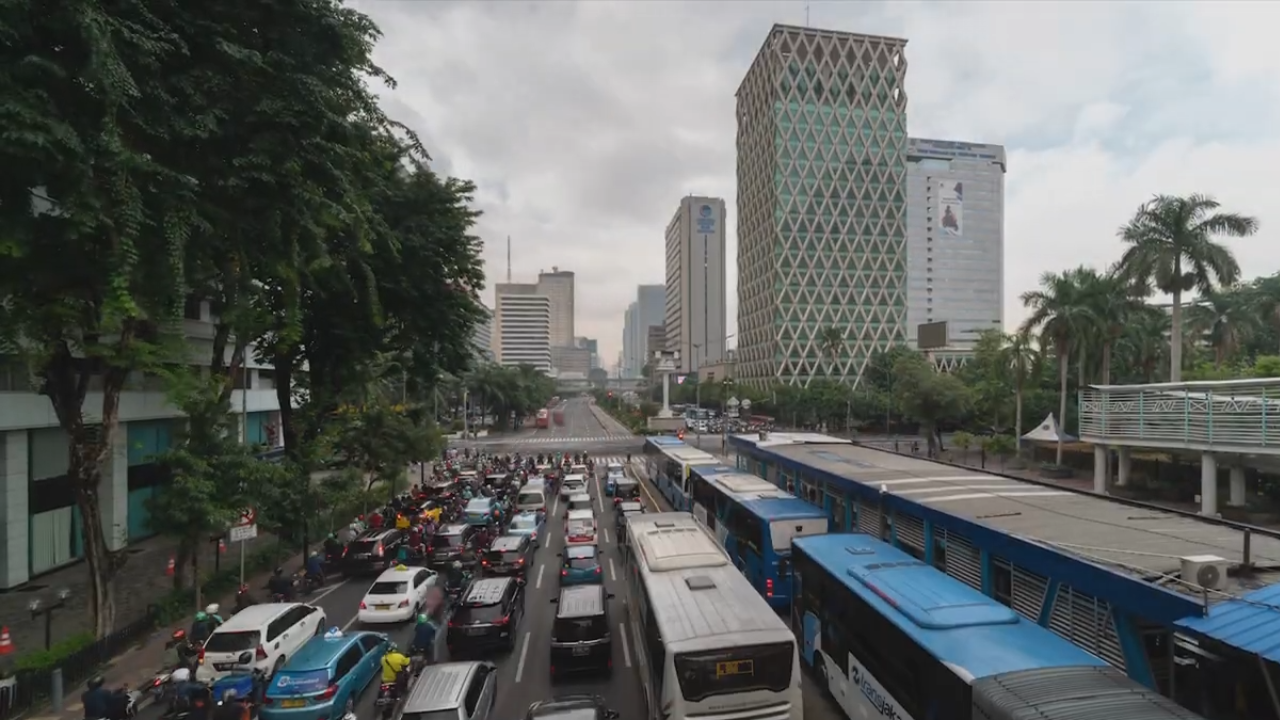
\includegraphics[width=0.8\linewidth, center]{images/input-image/input1.png}
    \caption{Contoh Frame dari \textit{source}.}
    \label{fig:input-image-rgb}
\end{afigure}

Penerapan filter spasial linear pada video \textit{stream} dilakukan dengan cara membaca setiap frame yang diterima dari \textit{source} sebagai citra digital, kemudian dilakukan filter spasial pada frame tersebut secara berkesinambungan. 
Salah satu contoh frame dari \textit{source} dapat dilihat pada gambar \ref{fig:input-image-rgb}. Selanjutnya frame tersebut dijadikan citra \textit{grayscale} sebelum dilakukan filter spasial, seperti pada gambar \ref{fig:input-grayscale}.

\begin{afigure}
    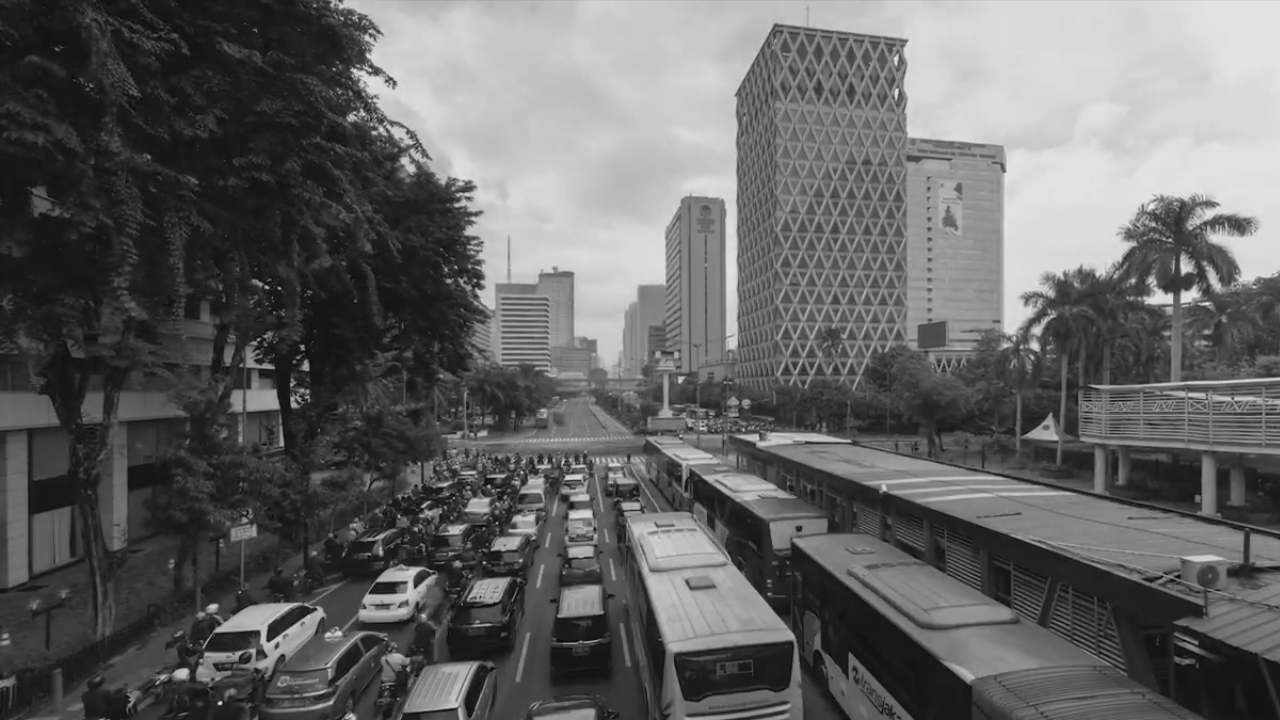
\includegraphics[width=0.8\linewidth, center]{images/output-image/input1-grayscale.png}
    \caption{Contoh Frame Grayscale.}
    \label{fig:input-grayscale}
\end{afigure}

\subsection{Average Blur}
Penerapan filter spasial pada frame \textit{grayscale} yang berukuran 1280x720 pixel dengan kernel \textit{average blur} (\ref{kernel:average}) yang berukuran 3x3 menghasilkan cita blur yang berukuran 1280x720. Hasil filter \textit{average blur} dapat dilihat pada gambar \ref{fig:output-averageblur}. Filter seperti ini dapat digunakan untuk mengurangi derau pada citra digital.
\begin{afigure}
    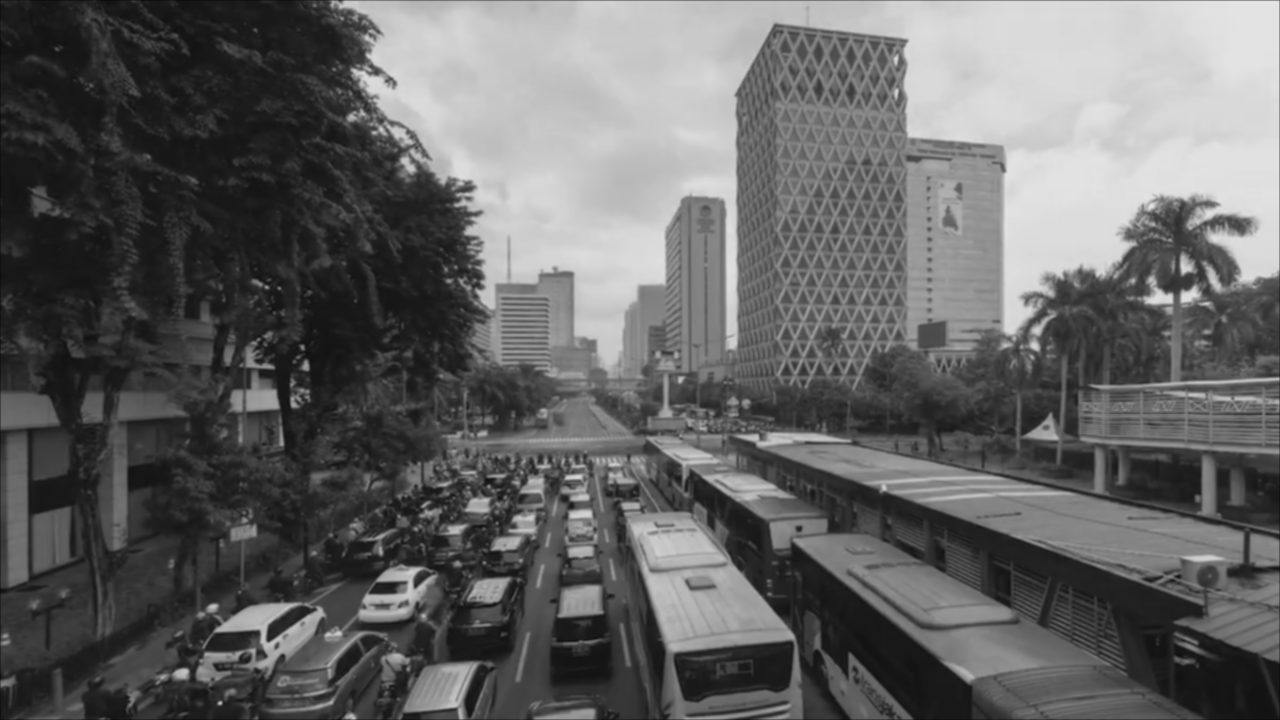
\includegraphics[width=0.8\linewidth, center]{images/output-image/input1-averageblur.png}
    \caption{Hasil filter Average Blur.}
    \label{fig:output-averageblur}
\end{afigure}

\subsection{Gaussian Blur}
Penerapan filter spasial dengan kernel \textit{gaussian blur} (\ref{kernel:gaussianblur}) yang berukuran 3x3 menghasilkan cita blur yang secara kasat mata hampir sama dengan filter \textit{average blur}. Namun apabila diperhatikan nilai masing-masing pixel pada gambar \ref{fig:output-gaussianblur} akan terlihat perbedaan dengan nilai masing-masing pixel pada gambar \ref{fig:output-averageblur}. Hal ini disebabkan karena nilai bobot pada kernel \textit{gaussian blur} (\ref{kernel:gaussianblur}). 
\begin{afigure}
    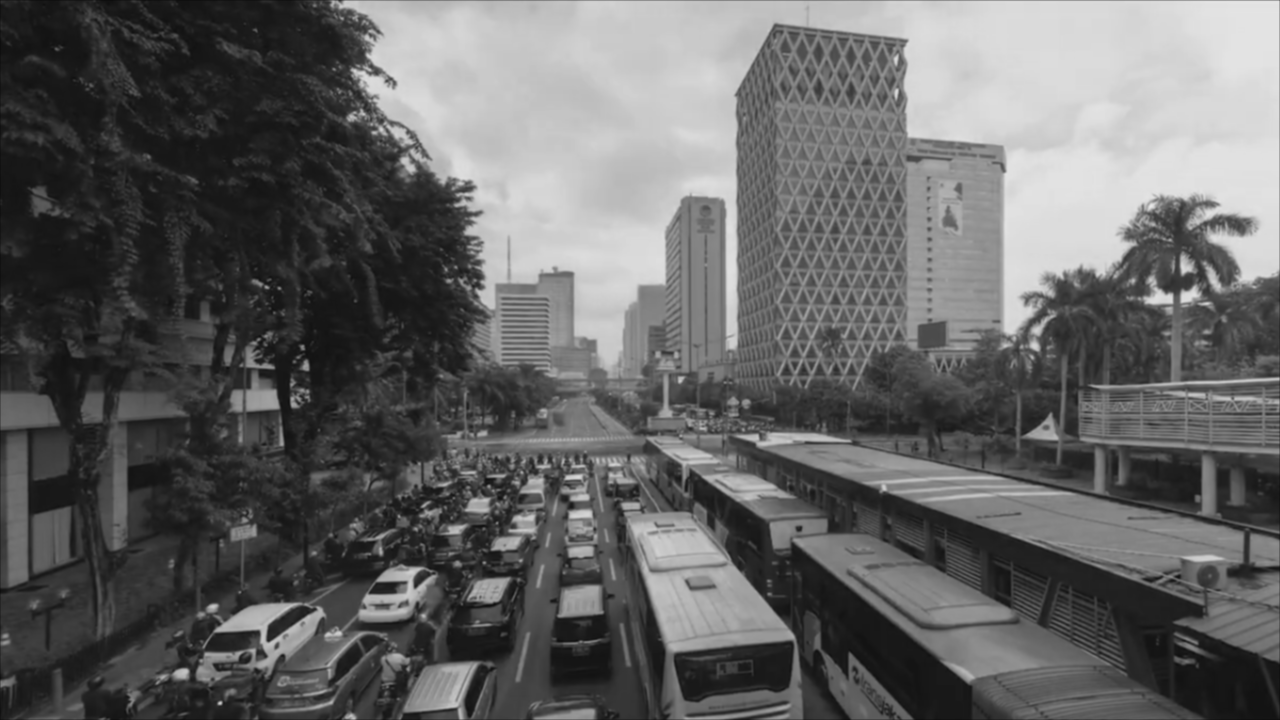
\includegraphics[width=0.8\linewidth, center]{images/output-image/input1-gaussianblur.png}
    \caption{Hasil filter Gaussian Blur.}
    \label{fig:output-gaussianblur}
\end{afigure}

\subsection{Laplacian}
Penerapan filter spasial dengan kernel \textit{laplacian} (\ref{kernel:laplacian}) menghasilkan cita biner, dapat dilihat pada gambar \ref{fig:output-laplacian}. Filter seperti ini dapat digunakan pada metode deteksi tepi di citra digital.
\begin{afigure}
    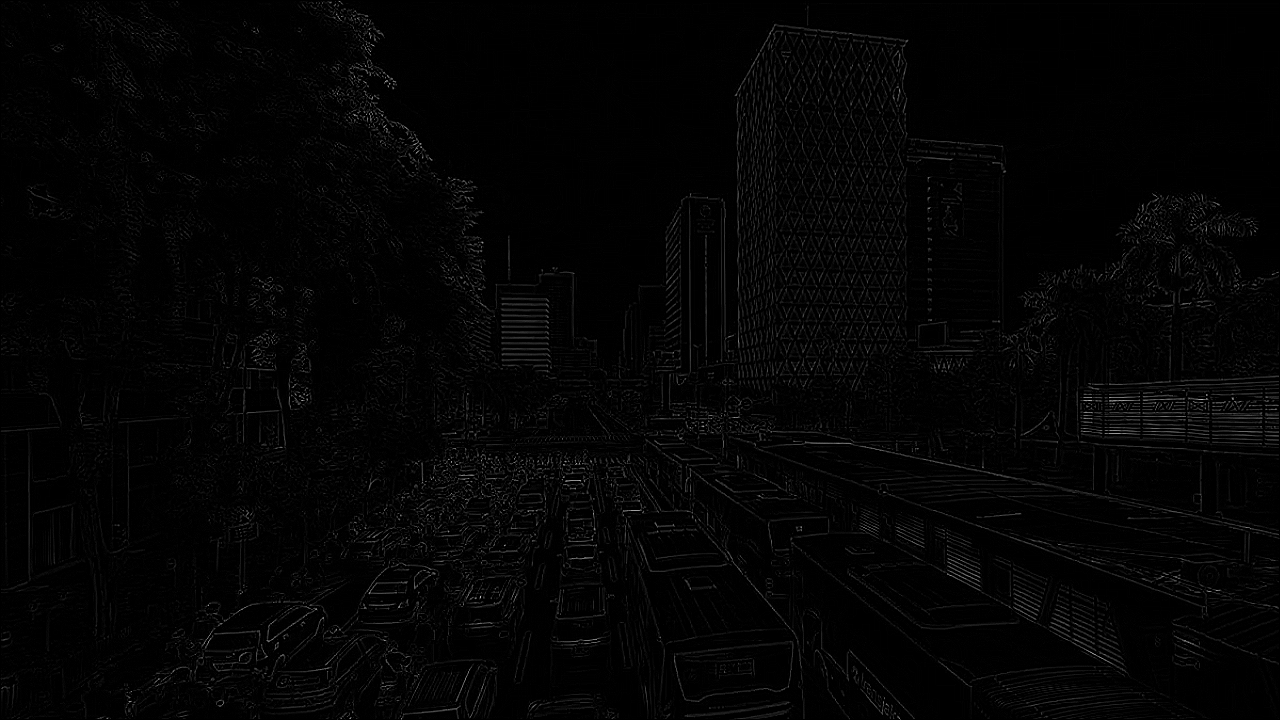
\includegraphics[width=0.8\linewidth, center]{images/output-image/input1-laplacian.png}
    \caption{Hasil filter Laplacian.}
    \label{fig:output-laplacian}
\end{afigure}

\subsection{Sharpening}
Penerapan filter spasial dengan kernel \textit{sharpening} (\ref{kernel:sharpen}) dapat meningkatkan detail (seperti garis) pada citra, namun dapat juga dapat menimbulkan derau pada citra apabila nilai kernelnya tidak sesuai. Filter seperti ini lebih tepat digunakan untuk memperbaiki kualitas citra (dengan nilai kernel yang sesuai). Hasil filter \textit{sharpening} ini dapat dilihat pada gambar \ref{fig:output-sharpen}.
\begin{afigure}
    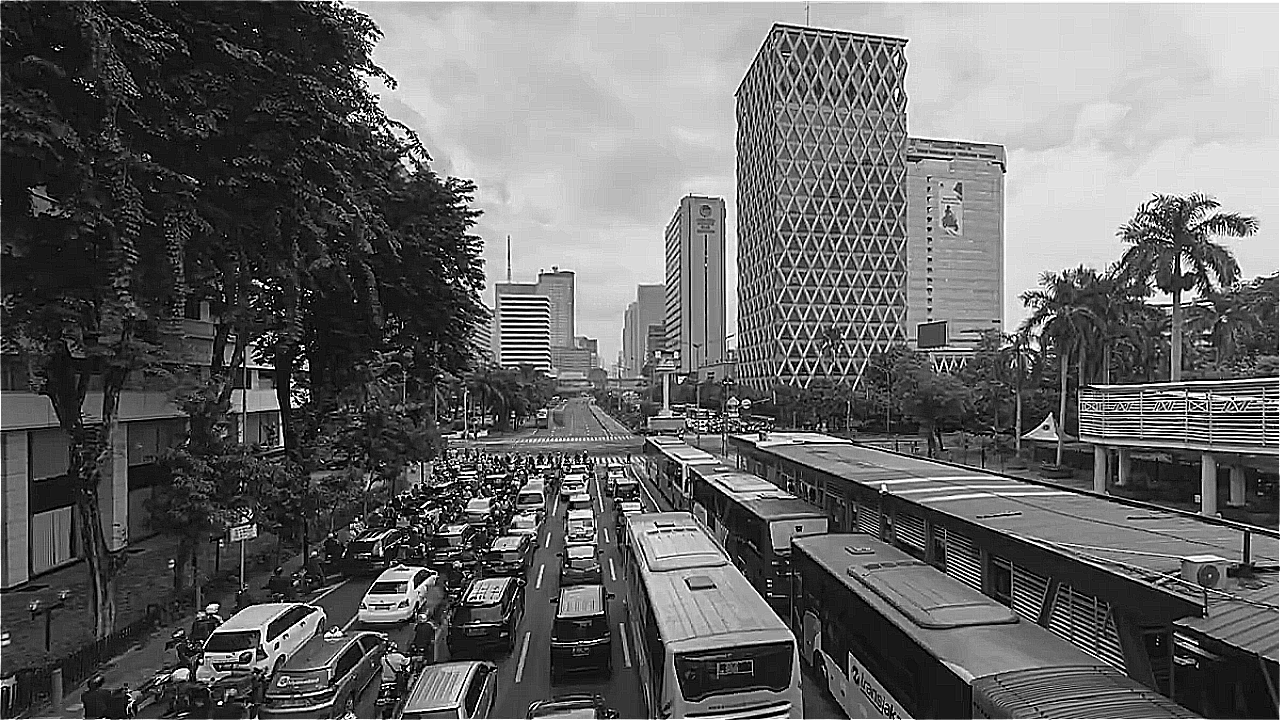
\includegraphics[width=0.8\linewidth, center]{images/output-image/input1-sharpen.png}
    \caption{Hasil filter Sharpening.}
    \label{fig:output-sharpen}
\end{afigure}

\subsection{Sobel Horizontal}
Penerapan filter spasial dengan kernel \textit{sobel horizontal} (\ref{kernel:sobel}) menghasilkan cita biner, dapat dilihat pada gambar \ref{fig:output-sobelhor}. Filter seperti lebih tepat digunakan pada metode deteksi tepi di citra yang banyak mengandung garis horizontal.
\begin{afigure}
    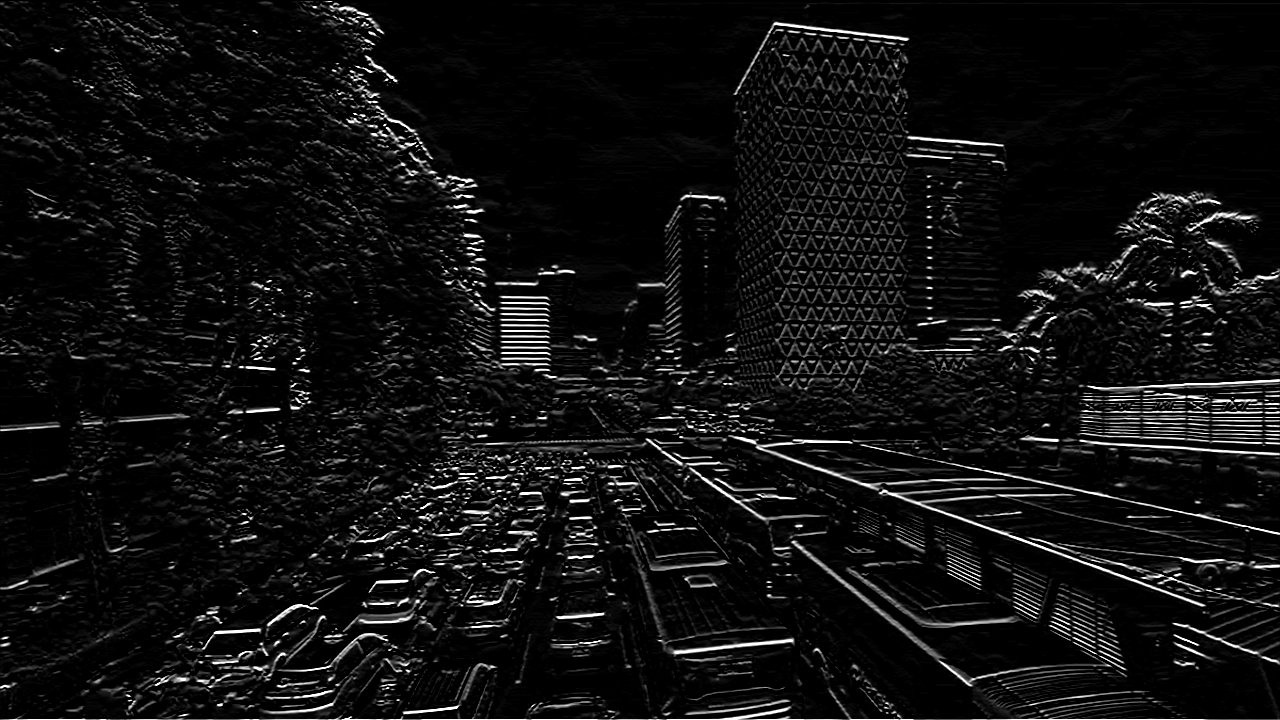
\includegraphics[width=0.8\linewidth, center]{images/output-image/input1-sobelhor.png}
    \caption{Hasil filter Sobel Horizontal.}
    \label{fig:output-sobelhor}
\end{afigure}

\subsection{Sobel Vertical}
Penerapan filter spasial dengan kernel \textit{sobel vertical} (\ref{kernel:sobel}) menghasilkan cita biner, dapat dilihat pada gambar \ref{fig:output-sobelver}. Sama halnya dengan filter \textit{sobel horizontal}, filter \textit{sobel vertical} juga dapat digunakan untuk metode deteksi tepi, terutama pada citra yang banyak mengandung garis verikal.
\begin{afigure}
    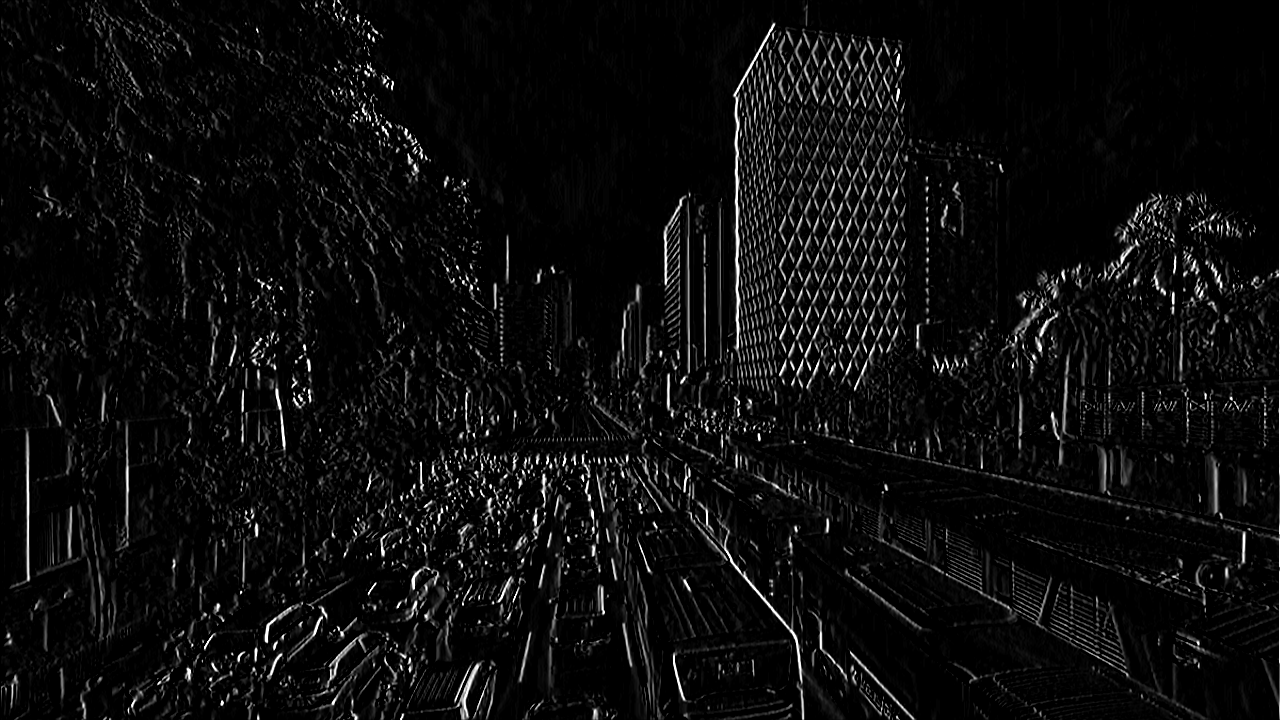
\includegraphics[width=0.8\linewidth, center]{images/output-image/input1-sobelver.png}
    \caption{Hasil filter Sobel Vertical.}
    \label{fig:output-sobelver}
\end{afigure}


% Jelaskan Proses Implementasi 
\section{Implementasi pada FPGA Development Board}
\blindtext
\subsection{Representasi Video Stream sebagai Citra Digital}
\subsection{Konversi Frame menjadi Grayscale}
\subsection{Penerapan Filter Spasial}
\subsubsection{Prosesor ARM}
\subsubsection{FPGA}
\subsection{Menghitung FPS}
\subsection{Mencatat Penggunaan Memory dan CPU}


% Jelaskan Hasil
\section{Analisis Kinerja}
\subsection{Waktu Komuptasi}
\begin{atable}
    \caption{Tabel perbandingan waktu komputasi dengan menggunakan 50 frame.}
    \label{table:hasil-time50}
    \csvreader[
        head to column names,
        tabular=lcc,
        separator=semicolon,
        before table=\rowcolors{2}{gray!15}{gray!30},
        table head= \rowcolor{gray!50!black} 
            \color{white} Filter & 
            \color{white} Prosesor ARM (s) & 
            \color{white} FPGA (s)\\]
        {tables/hasil-time50.csv}
        {filter=\filter, arm=\arm, fpga=\fpga}
        {\filter & \arm & \fpga }
\end{atable}
\blindtext
\begin{afigure}
    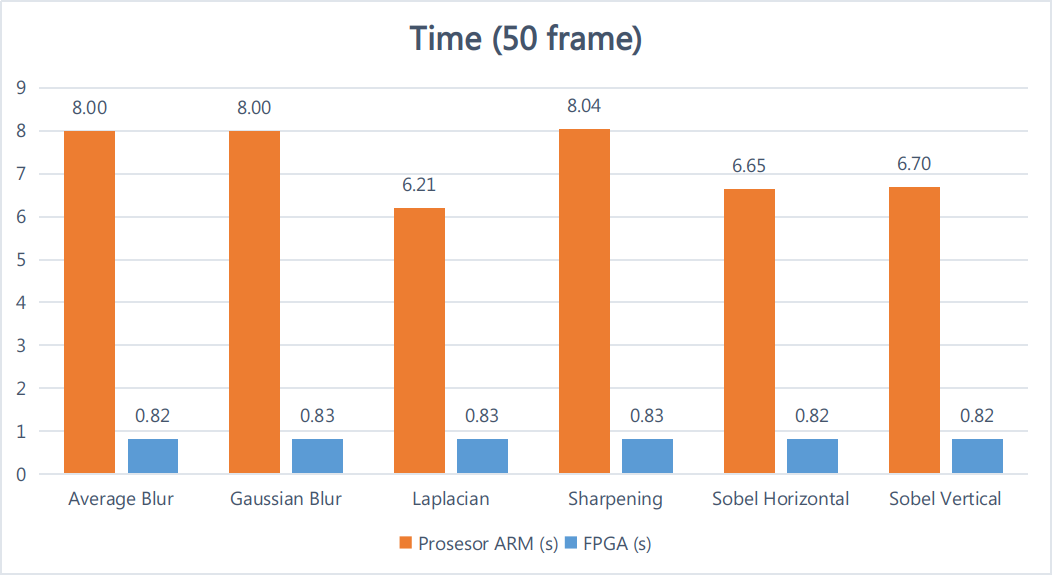
\includegraphics[width=0.9\linewidth, center]{images/chart/chart-time50.png}
    \caption{Grafik perbandingan waktu komputasi dengan menggunakan 50 frame.}
    \label{fig:chart-time50}
\end{afigure}


\subsection{Frame Rate (FPS)}
\begin{atable}
    \caption{Tabel perbandingan FPS dengan menggunakan prosesor ARM dan FPGA.}
    \label{table:hasil-fps}
    \csvreader[
        head to column names,
        tabular=lcc,
        before table=\rowcolors{2}{gray!15}{gray!30},
        table head= \rowcolor{gray!50!black} 
            \color{white} Filter & 
            \color{white} Tanpa FPGA & 
            \color{white} Dengan FPGA \\]
        {tables/hasil-fps.csv}
        {filter=\filter, tanpafpga=\tanpafpga, denganfpga=\denganfpga}
        {\filter & \tanpafpga & \denganfpga }
\end{atable}
\begin{afigure}
    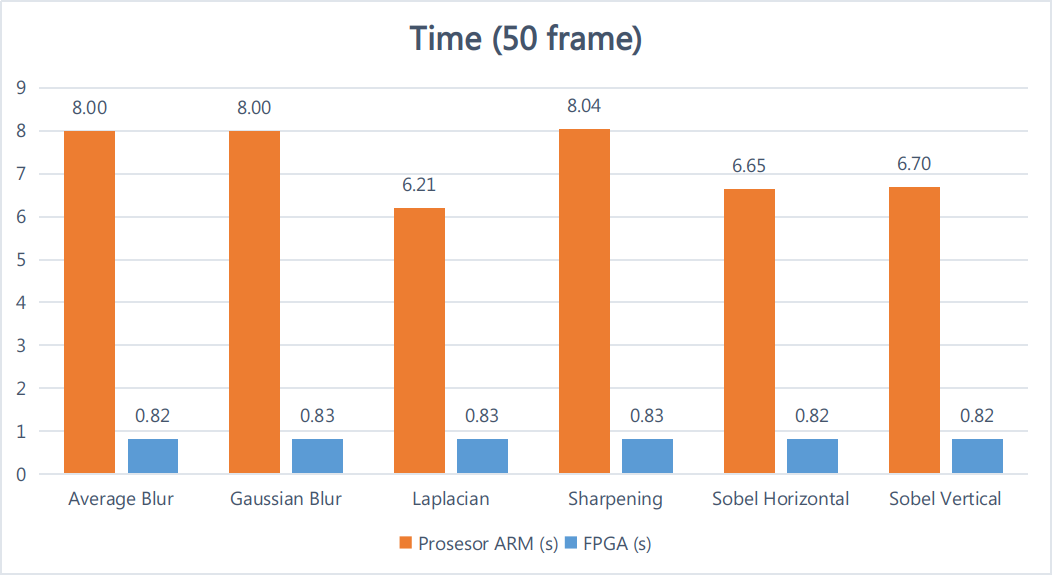
\includegraphics[width=0.9\linewidth, center]{images/chart/chart-time50.png}
    \caption{Grafik perbandingan FPS dengan menggunakan 50 frame.}
    \label{fig:chart-fps50}
\end{afigure}

\subsection{Penggunaan CPU}
\blindtext
\begin{afigure}
    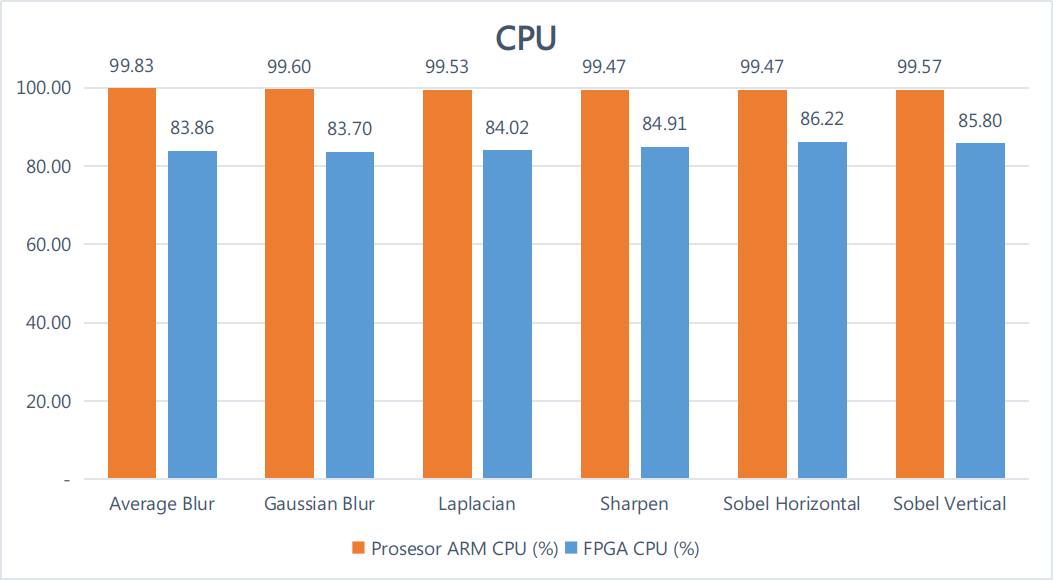
\includegraphics[width=0.9\linewidth, center]{images/chart/chart-cpu.png}
    \caption{Grafik perbandingan penggunaan CPU dengan menggunakan prosesor ARM dan FPGA.}
    \label{fig:chart-cpu}
\end{afigure}

\subsection{Penggunaan Memory}
\blindtext

\begin{afigure}
    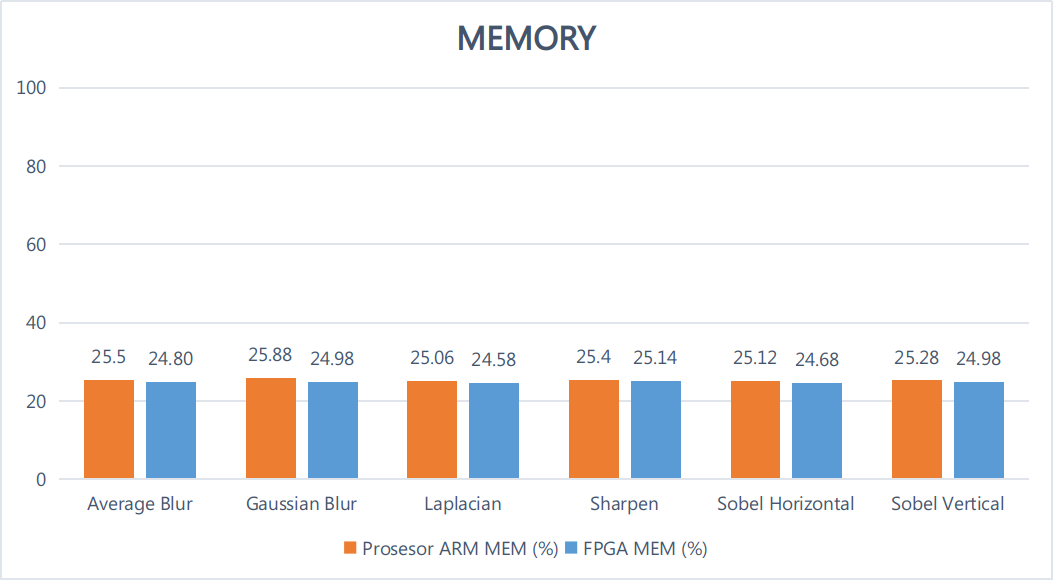
\includegraphics[width=0.9\linewidth, center]{images/chart/chart-mem.png}
    \caption{Grafik perbandingan penggunaan memory dengan menggunakan prosesor ARM dan FPGA.}
    \label{fig:chart-mem}
\end{afigure}

\subsection{Resident Memory (RES)}
\blindtext

\begin{afigure}
    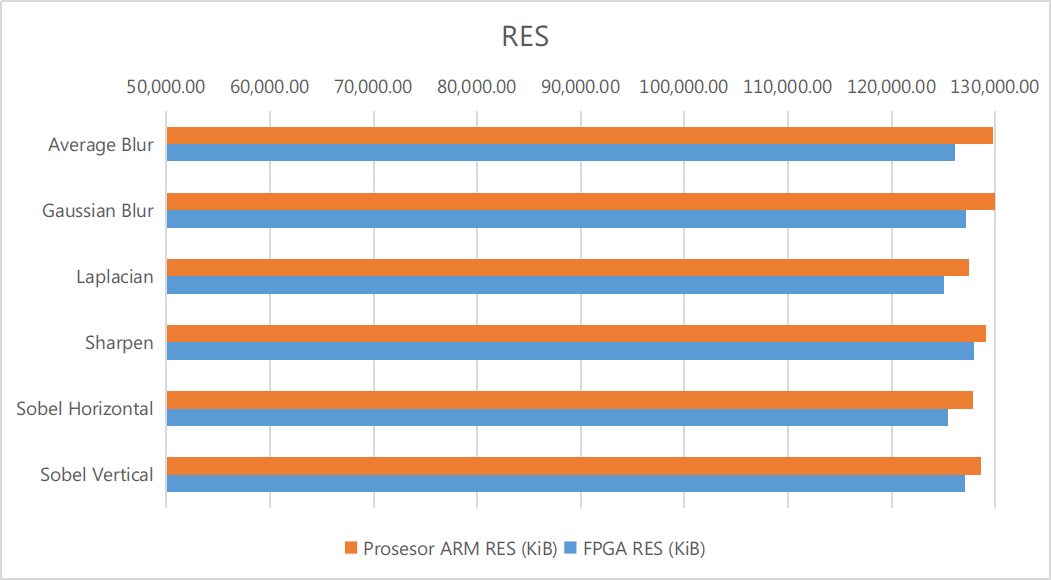
\includegraphics[width=0.9\linewidth, center]{images/chart/chart-res.png}
    \caption{Grafik perbandingan penggunaan resident memory dengan menggunakan prosesor ARM dan FPGA.}
    \label{fig:chart-res}
\end{afigure}

\subsection{Shared Memory (SHR)}
\blindtext

\begin{afigure}
    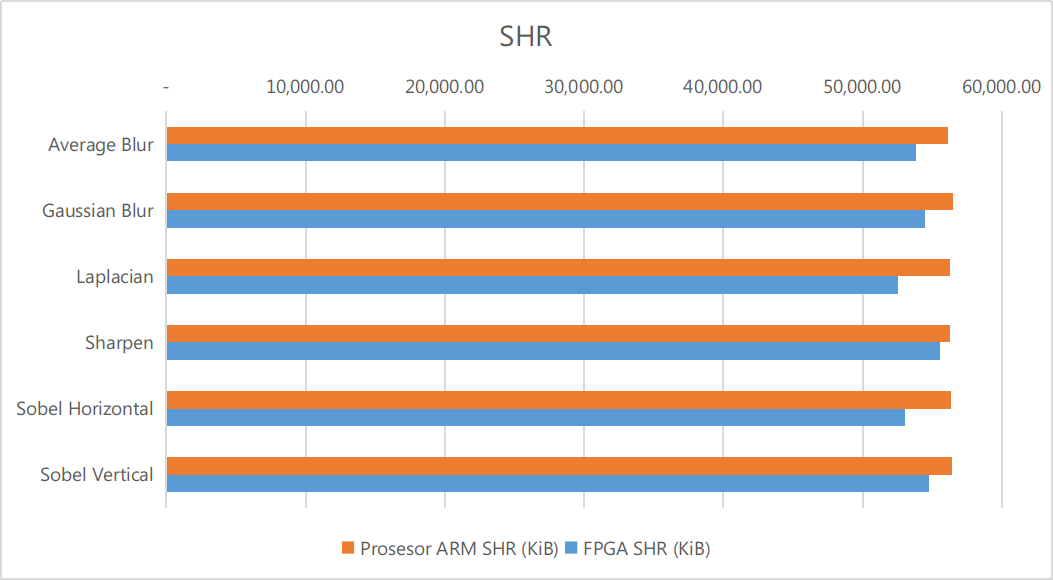
\includegraphics[width=0.9\linewidth, center]{images/chart/chart-shr.png}
    \caption{Grafik perbandingan penggunaan shared memory dengan menggunakan prosesor ARM dan FPGA.}
    \label{fig:chart-shr}
\end{afigure}

\subsection{Virtual Memory (VIRT)}
\blindtext

\begin{afigure}
    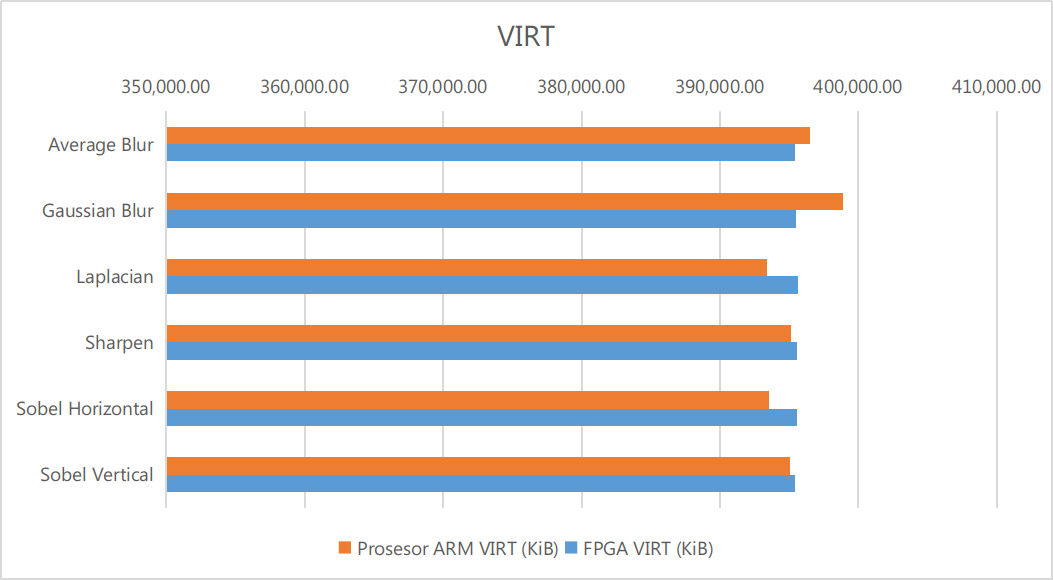
\includegraphics[width=0.9\linewidth, center]{images/chart/chart-virt.png}
    \caption{Grafik perbandingan penggunaan virtual memory dengan menggunakan prosesor ARM dan FPGA.}
    \label{fig:chart-virt}
\end{afigure}